% Transcription of Cayley's Collected Mathematical Papers, Vol. 9, pages 601--650
% Papers 623 (cont.), 624, 625, 626, 627, 628, 629
% Compiled from scanned images of the original Cambridge University Press edition

\documentclass[12pt,a4paper]{article}

% ------------------------------------------------------------------
% Standard English mathematical preamble
% ------------------------------------------------------------------
\usepackage[utf8]{inputenc}
\usepackage[T1]{fontenc}
\usepackage[english]{babel}
\usepackage{amsmath,amssymb,amsthm}
\usepackage{geometry}
\usepackage{fancyhdr}
\usepackage{titlesec}
\usepackage{enumitem}
\usepackage{array}
\usepackage{booktabs}
\usepackage{graphicx}
\usepackage{tikz}

\geometry{margin=1in}

% Custom commands for Cayley's notation
\newcommand{\xxi}{\xi}
\newcommand{\eeta}{\eta}
\DeclareMathOperator{\sn}{sn}
\DeclareMathOperator{\cn}{cn}
\DeclareMathOperator{\dn}{dn}

% For old-style fraction spacing
\newcommand{\fract}[2]{\frac{#1}{#2}}

% Page style
\pagestyle{fancy}
\fancyhf{}
\fancyhead[C]{\small CAYLEY---COLLECTED MATHEMATICAL PAPERS---VOL.\ IX}
\fancyfoot[C]{\thepage}
\renewcommand{\headrulewidth}{0.4pt}

% Section formatting (numbered paragraphs like original)
\renewcommand{\thesection}{\arabic{section}}
\titleformat{\section}{\large\bfseries\centering}{}{0em}{}
\titlespacing*{\section}{0pt}{2ex plus 1ex minus .2ex}{1ex plus .2ex}

% Subsection for internal divisions
\titleformat{\subsection}{\normalsize\bfseries\centering}{}{0em}{}
\titlespacing*{\subsection}{0pt}{1.5ex plus .5ex minus .2ex}{.5ex plus .2ex}

% Environment for displayed equations group
\newenvironment{eqns}{\[\begin{aligned}}{\end{aligned}\]}
\newenvironment{eqns*}{\[\begin{aligned}}{\end{aligned}\]}

% Compact list
\setlist{nosep}

\begin{document}

% ==================================================================
% PAPER 623 (continued) -- ON THREE-BAR MOTION
% Pages 579--580 of the volume = pages 601--602 of the PDF
% ==================================================================
\section*{623}
\subsection*{On Three-Bar Motion.\quad [Continued]}
\markboth{CAYLEY}{ON THREE-BAR MOTION}

\setcounter{equation}{0}
\noindent
that is,
\[
(b_1{}^{\!2} - a_2{}^{\!2})\, c\sigma - (c_1{}^{\!2} - a_3{}^{\!2})\, b\tau + \sigma\tau\, (c_1\tau - b_1\sigma) = 0,
\]
or, what is the same thing,
\[
(b_1{}^{\!2} - a_2{}^{\!2})\, c\sigma - (c_1{}^{\!2} - a_3{}^{\!2})\, b\tau + \sigma\tau\, (c\tau - b\sigma) = 0.
\]

Suppose, as in the figure, that $F$ is between $B$ and $A$; then, if $AF = \rho$, we have $c\tau = b\sigma + a\rho$, and the equation becomes
\[
(b_1{}^{\!2} - a_2{}^{\!2})\, c\sigma - (c_1{}^{\!2} - a_3{}^{\!2})\, b\tau + a\rho\sigma\tau = 0.
\]

Similarly, if, as in the figure, $G$ is on the other side of $A$, that is, between $A$ and $C$, and if $\rho'$, $\sigma'$, $\tau'$ be the distances $AG$, $BG$, $CG$, then $b\sigma' = c\tau' + a\rho'$, that is, $c\tau' - b\sigma' = -a\rho'$, and the corresponding equation is
\[
(b_1{}^{\!2} - a_2{}^{\!2})\, c\sigma' - (c_1{}^{\!2} - a_3{}^{\!2})\, b\tau' - a\rho'\sigma'\tau' = 0.
\]

We hence find
\begin{align*}
(b_1{}^{\!2} - a_2{}^{\!2})\, c\, (\sigma\tau' - \sigma'\tau) + a\tau\tau'\, (\rho\sigma + \rho'\sigma') &= 0, \\
(c_1{}^{\!2} - a_3{}^{\!2})\, b\, (\sigma\tau' - \sigma'\tau) + a\sigma\sigma'\, (\rho\tau + \rho'\tau') &= 0.
\end{align*}

But we have
\[
BG \cdot CF = BF \cdot CG + BC \cdot FG,
\]
that is,
\[
\sigma'\tau = \sigma\tau' + a \cdot FG, \quad \text{or } \sigma\tau' - \sigma'\tau = -a \cdot FG;
\]
also,
\[
\rho\sigma + \rho'\sigma' = AF \cdot BF + AG \cdot BG, \;= FG \cdot CH, \;= FG \cdot \tau'',
\]
and
\[
\rho\tau + \rho'\tau' = AF \cdot CF + AG \cdot CG, \;= FG \cdot BH, \;= FG \cdot \sigma'',
\]
as may be shown without difficulty, $\rho''$, $\sigma''$, $\tau''$ being the distances $AH$, $BH$, $CH$.
Hence the equations become
\begin{align*}
c\, (b_1{}^{\!2} - a_2{}^{\!2}) - \tau\tau'\tau'' &= 0, \\
b\, (c_1{}^{\!2} - a_3{}^{\!2}) - \sigma\sigma'\sigma'' &= 0,
\end{align*}

showing that, the foci being as in the figure, $b_1{}^{\!2} - a_2{}^{\!2}$ and $c_1{}^{\!2} - a_3{}^{\!2}$ are each of them positive; viz.\ that, in the generation by the triangle $OC_1B_1$, the radial bars $a_2$, $a_3$ are shorter than the sides $b_1$, $c_1$ respectively. Substituting for $b_1$, \&c.\ the values $k_1\sin B$, \&c.; also, instead of $k_1$, $k_2$, $k_3$, introducing the quantities $\lambda_1$, $\lambda_2$, $\lambda_3$, where
\[
k_1,\; k_2,\; k_3 = \lambda_1\sin A,\; \lambda_2\sin B,\; \lambda_3\sin C,
\]
these equations become
\begin{align*}
c\, (\lambda_1{}^{\!2} - \lambda_2{}^{\!2}) \sin^2 A \, \sin^2 B &= \tau\tau'\tau'', \\
b\, (\lambda_1{}^{\!2} - \lambda_3{}^{\!2}) \sin^2 A \, \sin^2 C &= \sigma\sigma'\sigma'';
\end{align*}
or, as these may be written, putting for shortness $M = \sin A \sin B \sin C$,
\begin{align*}
M^2 k^2\, (\lambda_1{}^{\!2} - \lambda_2{}^{\!2}) &= c\, \tau\tau'\tau'', \\
M^2 k^2\, (\lambda_1{}^{\!2} - \lambda_3{}^{\!2}) &= b\, \sigma\sigma'\sigma''.
\end{align*}

\vspace{1ex}
\noindent\rule{2em}{0.4pt}\hfill 73---2
\newpage

% ------------------------------------------------------------------
% Page 580 = PDF page 602
% ------------------------------------------------------------------
\noindent
All the quantities have so far been regarded as positive, and the formulae are applicable to the particular figure; but, to present them in a form applicable to any order of the nodes and foci, we have only to write the equations in the forms
\begin{align*}
M^2\, (\lambda_1{}^{\!2} - \lambda_2{}^{\!2}) &= k^2 \sin(\alpha-\beta) \sin(f-\gamma) \sin(g-\gamma) \sin(h-\gamma), \\
M^2\, (\lambda_1{}^{\!2} - \lambda_3{}^{\!2}) &= k^2 \sin(\alpha-\gamma) \sin(f-\beta) \sin(g-\beta) \sin(h-\beta);
\end{align*}
and these may be replaced by the system
\begin{align*}
M^2\, (\lambda_2{}^{\!2} - \lambda_3{}^{\!2}) &= k^2 \sin(\beta-\gamma) \sin(f-\alpha) \sin(g-\alpha) \sin(h-\alpha), \\
M^2\, (\lambda_3{}^{\!2} - \lambda_1{}^{\!2}) &= k^2 \sin(\gamma-\alpha) \sin(f-\beta) \sin(g-\beta) \sin(h-\beta), \\
M^2\, (\lambda_1{}^{\!2} - \lambda_2{}^{\!2}) &= k^2 \sin(\alpha-\beta) \sin(f-\gamma) \sin(g-\gamma) \sin(h-\gamma),
\end{align*}
since the first of these equations is implied in the other two; and then, reverting to the original form, we may write
\begin{align*}
M^2 k^2\, (\lambda_2{}^{\!2} - \lambda_3{}^{\!2}) &= BC \cdot FA \cdot GA \cdot HA, \\
M^2 k^2\, (\lambda_3{}^{\!2} - \lambda_1{}^{\!2}) &= CA \cdot FB \cdot GB \cdot HB, \\
M^2 k^2\, (\lambda_1{}^{\!2} - \lambda_2{}^{\!2}) &= AB \cdot FC \cdot GC \cdot HC,
\end{align*}
it being understood that the distances $BC$, $FA$, \&c., which enter into these equations, are not all positive, but that they stand for $k\sin(\beta-\gamma)$, $k\sin(f-\alpha)$, \&c., and that their signs are to be taken accordingly. Or, again, these may be written
\begin{align*}
BC\, (c_2{}^{\!2} - b_3{}^{\!2}) &= FA \cdot GA \cdot HA, \\
CA\, (a_3{}^{\!2} - c_1{}^{\!2}) &= FB \cdot GB \cdot HB, \\
AB\, (b_1{}^{\!2} - a_2{}^{\!2}) &= FC \cdot GC \cdot HC,
\end{align*}
where the signs are as just mentioned. We may say that $\pm\,(c_2{}^{\!2}-b_3{}^{\!2})$ is the modulus for the focus $A$; and the formula then shows that this modulus, taken positively, is equal to the product of the distances $FA$, $GA$, $HA$ of $A$ from the three nodes respectively, divided by $BC$, the distance of the other two foci from each other.

\newpage

% ==================================================================
% PAPER 624 -- ON THE BICURSAL SEXTIC
% Pages 581--587 of the volume = pages 603--609 of the PDF
% ==================================================================
\section*{624}
\subsection*{On the Bicursal Sextic.}
\markboth{CAYLEY}{ON THE BICURSAL SEXTIC}

\begin{center}
\small
[From the \textit{Proceedings of the London Mathematical Society}, vol.~VII. (1875---1876),\\
pp.~166---172.\quad Read March 10, 1876.]
\end{center}

\medskip
\noindent
In the paper ``On the mechanical description of certain sextic curves,'' \textit{Proceedings of the London Mathematical Society}, vol.~IV. (1872), pp.~105---111, [504], I obtained the bicursal sextic as a rational transformation of a binodal quartic. The theory was in effect as follows: taking $\Omega$, $P$, $Q$, $R$, each of them a function of $\lambda$, $\mu$ of the form $({}^*\!\!\mathbin{\backslash\!\!\backslash}\! 1,\lambda)^2(1,\mu)^2$, and considering $(\lambda,\,\mu)$ as connected by the equation $\Omega=0$, (viz.\ $\lambda$, $\mu$ being coordinates, this represents a binodal quartic), then, if we assume $x:y:z = P:Q:R$, the locus of the point $(x,\,y,\,z)$ is a curve rationally connected with the binodal quartic, viz.\ the points of the two curves have with each other a $(1,\,1)$ correspondence; whence the locus in question, say the curve $U=0$, is bicursal. The degree is obtained as the number of the intersections of the curve by an arbitrary line, or, what is the same thing, the number of the variable intersections of the corresponding $\lambda\mu$-curves
\[
\Omega = 0, \quad \alpha P + \beta Q + \gamma R = 0,
\]
viz.\ each of these being a quartic curve having the same two nodes, the nodes each count as 4 intersections, and the number of the remaining intersections is $4.4 - 2.4 = 8$, and thus the curve $U=0$ is in general of the order 8. But if the curves $\Omega=0$, $P=0$, $Q=0$, $R=0$ have (besides the nodes) $k$ common intersections, then these are also fixed intersections of the two curves $\Omega=0$, $\alpha P+\beta Q+\gamma R=0$, and the number of variable intersections is reduced to $8-k$; we have thus $8-k$ as the order of the curve $U=0$. In particular, if $k=2$, then the curve is a bicursal sextic.

The theory assumes a different and more simple form if, in the several functions $\Omega$, $P$, $Q$, $R$, we suppose that the terms in $\lambda^2$, $\mu^2$ are wanting. The curves $\Omega=0$, $P=0$, $Q=0$, $R=0$ are here cubics having two common points; the curve $U=0$, \textit{qui} rational transformation of the cubic $\Omega=0$, is still a bicursal curve; but its order is given as the number of the variable intersections of the cubics
\[
\Omega = 0, \quad \alpha P + \beta Q + \gamma R = 0,
\]
viz.\ this is $= 3.3 - 2 = 7$. But if the curves $\Omega=0$, $P=0$, $Q=0$, $R=0$ have (besides the before-mentioned two common points) $k$ other common points, then the number of the variable intersections is $=7-k$: and this is therefore the order of the curve $U=0$. In particular, if $k=1$, then the curve is a bicursal sextic. And, in the present paper, I consider the binodal sextic as thus obtained, viz.\ as given by the equations $\Omega=0$, $x:y:z = P:Q:R$, where $\Omega=0$, $P=0$, $Q=0$, $R=0$ are cubics, having (in all) three common points.

The bicursal sextic has in general 9 nodes; but 3 of these may unite together into a triple point: this will be the case if, in the series of curves $\alpha P + \beta Q + \gamma R = 0$, there are any two curves which have 3 common intersections with the curve $\Omega=0$. (Observe that we throughout disregard the 3 common points of the curves $\Omega=0$, $P=0$, $Q=0$, $R=0$, and attend only to the 6 variable points of intersection of the curves $\Omega=0$ and $\alpha P+\beta Q+\gamma R=0$,---the meaning is, that there are two curves of the series such that, attending only to the 6 variable intersections of each of them with the curve $\Omega=0$, there are three common intersections.) For, supposing the two curves to be $\alpha P+\beta Q+\gamma R=0$ and $\alpha' P+\beta' Q+\gamma' R=0$, then any curve whatever
\[
\alpha P + \beta Q + \gamma R + \theta\, (\alpha' P + \beta' Q + \gamma' R) = 0
\]
has the same three intersections with the curve $\Omega=0$, say these are the points $A_1$, $A_2$, $A_3$, the coordinates of which are independent of $\theta$. Hence the line
\[
(\alpha x + \beta y + \gamma z) + \theta\, (\alpha' x + \beta' y + \gamma' z) = 0
\]
intersects the curve $U=0$ in six points, three of which, as corresponding to the points $A_1$, $A_2$, $A_3$, are independent of $\theta$, viz.\ they are the same three points for any line whatever of the series; and this means that the curve $U=0$ has at the point
\[
(\alpha x + \beta y + \gamma z = 0,\quad \alpha' x + \beta' y + \gamma' z = 0)
\]
a triple point; and that to this triple point correspond the three points $A_1$, $A_2$, $A_3$.

We may, in the series of lines $\alpha x+\beta y+\gamma z + \theta(\alpha' x+\beta' y+\gamma' z)=0$, rationally determine $\theta$ so that one of the three variable points of intersection shall correspond to $A_1$, $A_2$, or $A_3$; viz.\ $\theta$ must be such that the curve $\alpha P+\beta Q+\gamma R+\theta(\alpha' P+\beta' Q+\gamma' R)=0$ shall touch the curve $\Omega=0$ at one of the points $A_1$, $A_2$, $A_3$. The three lines thus determined are the three tangents to the curve at the triple point: and the three branches may be considered as corresponding to the three points $A_1$, $A_2$, $A_3$, respectively.

There is no loss of generality in assuming that the triple point is the point $(x=0,\; z=0)$; the condition then simply is that the curves $P=0$, $R=0$ shall have three common intersections with the curve $\Omega=0$; and the tangents at the triple point are $x+\theta z=0$, $\theta$ being so determined that one of the three variable points of intersection shall correspond to one of the three points $A_1$, $A_2$, $A_3$: in particular, if this is the case for the line $x=0$, then this line will be one of the tangents at the triple point.

\newpage

% ------------------------------------------------------------------
% Page 583 = PDF page 605
% ------------------------------------------------------------------
\noindent
The bicursal sextic may have a second triple point, viz.\ three other nodes may unite together into a triple point. The theory is precisely the same: we must have two other curves $\alpha P+\beta Q+\gamma R=0$, $\alpha' P+\beta' Q+\gamma' R=0$, having with the curve $\Omega=0$ three common intersections $B_1$, $B_2$, $B_3$: there is then a second triple point
\[
(\alpha x + \beta y + \gamma z = 0,\quad \alpha' x + \beta' y + \gamma' z = 0);
\]
and, to find the tangents at this point, we must determine $\theta$ so that one of the variable points of intersection of the line
\[
\alpha x + \beta y + \gamma z + \theta\, (\alpha' x + \beta' y + \gamma' z) = 0
\]
with the sextic shall correspond with $B_1$, $B_2$, or $B_3$; viz.\ $\theta$ must be such that the curve $\alpha P+\beta Q+\gamma R+\theta(\alpha' P+\beta' Q+\gamma' R)=0$ shall touch the curve $\Omega=0$ at one of the points $B_1$, $B_2$, $B_3$. In particular, if, as before, the curves $P=0$, $R=0$ have three common intersections with the curve $\Omega=0$, and if, moreover, the curves $Q=0$, $R=0$ have three common intersections with the curve $\Omega=0$, then the bicursal sextic will have the two triple points $(x=0,\; z=0)$ and $(y=0,\; z=0)$; and it may further happen that the line $x=0$ is a tangent at the first triple point, and the line $y=0$ a tangent at the second triple point. The sextic may in like manner have a third triple point, but this is a special case which I do not at present consider.

I write for greater convenience $\dfrac{\lambda}{\nu}$, $\dfrac{\mu}{\nu}$ in place of $\lambda$, $\mu$, so as to make $\Omega$, $P$, $Q$, $R$ each of them a homogeneous cubic function of $(\lambda,\,\mu,\,\nu)$; and I give to these functions, not the most general values belonging to a bicursal sextic with two triple points, but the values in the form obtained for them, as appearing further on, in the problem of three-bar motion; viz.\ the equations $\Omega=0$, $x:y:z = P:Q:R$ are respectively taken to be
\begin{align*}
\nu\,(h\nu\lambda + f\lambda^2) + \mu\,(g\nu^2 + e\nu\lambda + g\lambda^2) + \mu^2\,(f\nu + h\lambda) &= 0, \\
x:y:z = \lambda\mu\,(a\lambda+b\mu) : \nu^2(c\lambda+d\mu) : \lambda\mu\nu&.\phantom{=0}
\end{align*}

The four curves $\Omega=0$, $P=0$, $Q=0$, $R=0$ have thus the three common intersections
\[
(\mu=0,\; \nu=0),\quad (\nu=0,\; \lambda=0),\quad (\lambda=0,\; \mu=0),
\]
represented in the figure by the points $A$, $B$, $C$; the curve drawn in the figure is the curve $\Omega=0$, and the points $F$, $G$, $H$ are the third points of intersection of the cubic with the lines $BC$, $CA$, $AB$ respectively.

\begin{center}
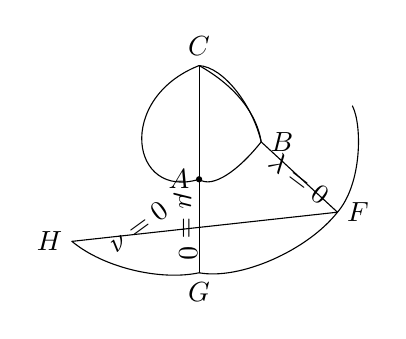
\begin{tikzpicture}[scale=0.95,line cap=round,line join=round]
  \coordinate (C) at (0,1.32);
  \coordinate (A) at (0,-0.20);
  \coordinate (G) at (0,-1.45);
  \coordinate (H) at (-1.70,-1.03);
  \coordinate (B) at (0.83,0.30);
  \coordinate (F) at (1.85,-0.64);

  \draw (C) -- (G);
  \draw (H) -- (F);
  \draw (B) -- (F);

  \draw
    (H) .. controls (-1.28,-1.38) and (-0.52,-1.56) .. (G)
        .. controls (0.55,-1.55) and (1.45,-1.15) .. (F)
        .. controls (2.18,-0.26) and (2.18,0.53) .. (2.05,0.78);
  \draw
    (A) .. controls (-0.92,-0.48) and (-1.12,0.88) .. (C)
        .. controls (0.33,1.30) and (0.72,0.78) .. (B)
        .. controls (0.53,-0.08) and (0.18,-0.33) .. (A);
  \draw (C) .. controls (0.52,1.03) and (0.78,0.64) .. (B);

  \fill (A) circle (1.2pt);
  \node[above] at (C) {$C$};
  \node[left] at (A) {$A$};
  \node[right] at (B) {$B$};
  \node[below] at (G) {$G$};
  \node[left] at (H) {$H$};
  \node[right] at (F) {$F$};

  \node[rotate=-90] at (-0.18,-0.83) {$\mu=0$};
  \node[rotate=36] at (-0.82,-0.83) {$\nu=0$};
  \node[rotate=-37] at (1.34,-0.18) {$\lambda=0$};
\end{tikzpicture}
\end{center}

The equation $P+\theta R=0$ is here $\lambda\mu\,(a\lambda+b\mu+\theta\nu)=0$, which intersects $\Omega=0$ in the points $C$, $A$, $G$, $C$, $B$, $F$, and the three intersections by the line $a\lambda+b\mu+\theta\nu=0$;

\newpage

% ------------------------------------------------------------------
% Page 584 = PDF page 606
% ------------------------------------------------------------------
\noindent
viz.\ excluding the fixed points $A$, $B$, $C$, the six intersections are $C$, $F$, $G$, and the three intersections by the line. Hence, of the six intersections, we have $C$, $F$, $G$ independent of $\theta$, or we have $(x=0,\; z=0)$ a triple point, say $I$, corresponding to the three points $C$, $F$, $G$, viz.\ these are the points
\[
(\lambda,\,\mu,\,\nu) = (0,\,0,\,1),\quad (0,\,g,\,-f),\quad (h,\,0,\,-f), \qquad (C,\,F,\,G).
\]

The equation $Q+\theta R=0$ is $\nu\,(c\lambda\nu+d\mu\nu+\theta\lambda\mu)=0$; viz.\ the line $\nu=0$ meets $\Omega=0$ in the three points $A$, $B$, $H$, and the conic $c\lambda\nu+d\mu\nu+\theta\lambda\mu=0$ meets $\Omega=0$ in the points $A$, $B$, $C$, and three other points: hence, rejecting the points $A$, $B$, $C$, the six points of intersection are the points $A$, $B$, $H$, and the three variable points of intersection by the conic; or we have $(y=0,\; z=0)$ a triple point, say $J$, corresponding to the three points $A$, $B$, $H$, viz.\ these are the points
\[
(\lambda,\,\mu,\,\nu) = (1,\,0,\,0),\quad (0,\,1,\,0),\quad (h,\,-g,\,0), \qquad (A,\,B,\,H).
\]

To find the tangents at the triple point $I$, these are $x+\theta z=0$, where $\theta$ is to be successively determined by the conditions that the line $a\lambda+b\mu+\theta\nu=0$ shall pass through the points $C$, $F$, $G$*; viz.\ we thus have
\begin{alignat*}{3}
\theta &= 0, &\qquad x &= 0, \quad \text{the tangent corresponding to the point } C,\; (0,\,0,\,1), \\
\theta &= +\frac{bg}{f}, &\qquad fx+bgz &= 0, \quad\;\, \text{``\quad\quad\quad\quad\quad\quad\quad\quad\quad\quad\quad\quad\quad\quad\quad\quad\quad\quad} F,\; (0,\,g,\,-f), \\
\theta &= +\frac{ah}{f}, &\qquad fx+ahz &= 0, \quad\;\, \text{``\quad\quad\quad\quad\quad\quad\quad\quad\quad\quad\quad\quad\quad\quad\quad\quad\quad\quad} G,\; (h,\,0,\,-f).
\end{alignat*}

And similarly, at the triple point $J$, the tangents are $y+\theta z=0$, where $\theta$ is to be successively determined by the conditions that the conic $c\nu\lambda+d\nu\mu+\theta\lambda\mu=0$ shall pass through the point $H$, and shall touch the cubic at the points $A$, $B$; viz.\ we thus have
\begin{alignat*}{3}
\theta &= 0, &\qquad y &= 0, \quad \text{the tangent corresponding to the point } H,\; (h,\,-g,\,0), \\
\theta &= \frac{cg}{f}, &\qquad fy+cgz &= 0, \quad\;\, \text{``\quad\quad\quad\quad\quad\quad\quad\quad\quad\quad\quad\quad\quad\quad\quad\quad\quad\quad} A,\; (1,\,0,\,0), \\
\theta &= \frac{dh}{f}, &\qquad fy+dhz &= 0, \quad\;\, \text{``\quad\quad\quad\quad\quad\quad\quad\quad\quad\quad\quad\quad\quad\quad\quad\quad\quad\quad} B,\; (0,\,1,\,0).
\end{alignat*}

The two last values of $\theta$ are obtained by the consideration that the equations of the tangents to $\Omega=0$ at the points $A$, $B$ respectively, are $g\mu+f\nu=0$, $h\lambda+f\nu=0$, where $\lambda$, $\mu$, $\nu$ are current coordinates of a point on the tangent: it may be added that the equation of the tangent at the point $C$ is $h\lambda+g\mu=0$.

\vspace{1ex}
\noindent\rule{2em}{0.4pt}
\begin{flushleft}
\small
* Observe the somewhat altered form of the condition: $\theta$ is to be determined so that the cubic $\lambda\mu\,(a\lambda+b\mu+\theta\nu)=0$ shall touch the cubic $\Omega=0$ at one of the points $C$, $F$, $G$: but, as the first-mentioned cubic breaks up, and the component curve $a\lambda+b\mu+\theta\nu=0$ does not pass through any one of these points, this can only mean that $\theta$ shall be so determined as that the line shall pass through one of these points, viz.\ that there shall be at the point, not a proper contact, but a double intersection, arising from a node of the cubic $\lambda\mu\,(a\lambda+b\mu+\theta\nu)=0$. And the like case happens for the other triple point; viz.\ there the cubic $\nu\,(c\nu\lambda+d\nu\mu+\theta\lambda\mu)=0$ is to touch the cubic $\Omega=0$ at one of the points $A$, $B$, $H$; the component conic $c\nu\lambda+d\nu\mu+\theta\lambda\mu=0$ passes through the points $A$ and $B$ but not through $H$; hence the conditions for $\theta$ are, that the conic shall touch the cubic at $A$ or $B$, or that it shall pass through $H$.
\end{flushleft}

\newpage

% ------------------------------------------------------------------
% Page 585 = PDF page 607
% ------------------------------------------------------------------
\noindent
The three-bar curve may be represented by means of a system of equations of the last-mentioned form, viz.\ $x:y:z = \lambda\mu\,(a\lambda+b\mu) : \nu^2(c\lambda+d\mu) : \lambda\mu\nu$, where $\lambda$, $\mu$, $\nu$ are connected as above; or, taking $X$, $Y$ as ordinary rectangular coordinates, $x$, $y$, and $z$ are here the circular coordinates $\dfrac{x}{z} = X+iY$, $\dfrac{y}{z} = X-iY$, and $z=1$; and the parameters $\dfrac{\lambda}{\nu}$, $\dfrac{\mu}{\nu}$ denote like functions $\cos\theta+i\sin\theta$, $\cos\phi+i\sin\phi$ of angles which are the inclinations of two bars to a fixed line. Using, for convenience, Figure 2 of my paper on Three-bar Motion, (p.~553 of this volume), the curve is considered as the locus of the vertex $O$ of the triangle $OC_1B_1$, connected by the bars $C_1C$ and $B_1B$ with the fixed points $B$ and $C$ respectively; and we have $CC_1=a_2$, $OC_1=b_1$, $OB_1=c_1$, $C_1B_1=a_1$, $B_1B=a_3$. Also, to avoid confusion with the foregoing notation of the present paper, instead of calling it $a$, I take $BC=a_0$: the angle $OC_1B_1$ is $=C_1$, and $\cos C_1+i\sin C_1$ is taken $=\gamma$.

Hence, taking the origin at $C$, the axis of $X$ coinciding with $CB$ and that of $Y$ being at right angles to it: taking also $\theta$, $\phi$, $\psi$ for the inclinations of $CC_1$, $C_1B_1$, and $B_1B$ to $CB$, we have
\begin{alignat*}{2}
a_2\cos\theta + a_1\cos\phi - a &= -a_3\cos\psi, \\
a_2\sin\theta + a_1\sin\phi &\hphantom{{}={}} = \hphantom{-}a_3\sin\psi;
\end{alignat*}
viz.\ writing $\cos\theta+i\sin\theta=\lambda$, $\cos\phi+i\sin\phi=\mu$, these give
\begin{align*}
a_2\lambda + a_1\mu - a_0 &= -a_3\,(\cos\psi - i\sin\psi), \\
a_2\frac{1}{\lambda} + a_1\frac{1}{\mu} - a_0 &= -a_3\,(\cos\psi + i\sin\psi),
\end{align*}
that is,
\[
(a_2\lambda + a_1\mu - a)\,\bigl(a_2\frac{1}{\lambda} + a_1\frac{1}{\mu} - a_0\bigr) - a_3{}^{\!2} = 0;
\]
viz.
\[
(a_0{}^{\!2} + a_1{}^{\!2} + a_2{}^{\!2} - a_3{}^{\!2}) + a_1a_2\,\Bigl(\frac{\mu}{\lambda}+\frac{\lambda}{\mu}\Bigr) - a_0a_2\,\Bigl(\lambda+\frac{1}{\lambda}\Bigr) - a_0a_1\,\Bigl(\mu+\frac{1}{\mu}\Bigr) = 0,
\]
for the relation between the parameters $\lambda$, $\mu$. And then
\begin{align*}
X &= a_2\cos\theta + b_1\cos(\phi+C_1), \\
Y &= a_2\sin\theta + b_1\sin(\phi+C_1);
\end{align*}
viz.\ if $x$, $y = X+iY$, $X-iY$, then
\[
\begin{cases}
x = a_2\lambda + b_2\gamma_1\mu, \\[4pt]
y = a_2\dfrac{1}{\lambda} + b_2\dfrac{1}{\gamma_1\mu},
\end{cases}
\]
which equations determine the coordinates $(x,\,y)$ in terms of the parameters $\lambda$, $\mu$ connected by the foregoing relation.

\vspace{1ex}
\noindent\rule{2em}{0.4pt}\hfill 74

\newpage

% ------------------------------------------------------------------
% Page 586 = PDF page 608
% ------------------------------------------------------------------
\noindent
Writing for homogeneity $\dfrac{\lambda}{\nu}$, $\dfrac{\mu}{\nu}$ in place of $\lambda$, $\mu$, and $\dfrac{x}{z}$, $\dfrac{y}{z}$ in place of $x$, $y$, the equations become
\[
(a_0{}^{\!2} + a_1{}^{\!2} + a_2{}^{\!2} - a_3{}^{\!2})\,\lambda\mu\nu + a_1a_2\,(\lambda^2+\mu^2)\,\nu - a_0a_2\mu\,(\nu^2+\lambda^2) - a_0a_1\lambda\,(\mu^2+\nu^2) = 0,
\]
and
\[
x:y:z = (a_2\lambda + b_2\gamma_1\mu)\,\lambda\mu : \Bigl(\frac{b_2}{\gamma_1}\lambda + a_2\mu\Bigr)\,\nu^2 : \lambda\mu\nu.
\]

Comparing with the foregoing equations
\[
e\,\lambda\mu\nu + f(\lambda^2+\mu^2)\,\nu + g(\nu^2+\lambda^2)\,\mu + h(\mu^2+\nu^2)\,\lambda = 0,
\]
and
\[
x:y:z = (a\lambda+b\mu)\,\lambda\mu : (c\lambda+d\mu)\,\nu^2 : \lambda\mu\nu,
\]
the equations agree together, and we have
\[
\left\{\begin{aligned}
e &= a_0{}^{\!2} + a_1{}^{\!2} + a_2{}^{\!2} - a_3{}^{\!2}, \\
f &= +a_1a_2, \\
g &= -a_0a_2, \\
h &= -a_0a_1, \\
a &= \hphantom{+}a_2, \\
b &= \hphantom{+}b_1\gamma_1, \\
c &= \hphantom{+}\frac{b_1}{\gamma_1}, \\
d &= \hphantom{+}a_2.
\end{aligned}\right.
\]

The tangents at the triple points thus are
\[
\begin{array}{c@{\	ext{\qquad}}c}
x = 0, & y = 0, \\[4pt]
a_1x - a_0b_1\gamma_1 z = 0, & a_1y - \dfrac{a_0b_1}{\gamma_1} z = 0, \\[6pt]
x - a_0z = 0, & y - a_0z = 0;
\end{array}
\]
viz.\ restoring the rectangular coordinates, and for $\gamma$ substituting the value $\cos C + i\sin C$, for $a_0$ writing $a$, and taking $b = \dfrac{ab_1}{a_1}$, we have
\[
\begin{array}{c@{\	ext{\qquad}}c}
X + iY = 0, & X - iY = 0, \\[4pt]
X + iY = b\, (\cos C + i\sin C), & X - iY = b\, (\cos C - i\sin C), \\[4pt]
X + iY = a_0, & X - iY = a_0;
\end{array}
\]
viz.\ the first two intersect in the point $(0,\,0)$, the second two in the point $(b\cos C,\; b\sin C)$, the third two in the point $(a,\,0)$: the first and third of these are the points $B$ and $C$, the second of them is the point $A$ of the figure; viz.\ the formulae give the point $A$, forming, with $B$ and $C$, a triad of foci.

\newpage


% ==================================================================
% PAPER 625 -- ON THE CONDITION FOR THE EXISTENCE OF A SURFACE
% Pages 587--592 of the volume = pages 609--614 of the PDF
% ==================================================================
\section*{625}
\subsection*{On the Condition for the Existence of a Surface Cutting at Right Angles a Given Set of Lines.}
\markboth{CAYLEY}{ON THE CONDITION FOR THE EXISTENCE OF A SURFACE}

\begin{center}
\small
[From the \textit{Proceedings of the London Mathematical Society}, vol.~VIII. (1876---1877),\\
pp.~53---57.\quad Read December 14, 1876.]
\end{center}

\medskip
\noindent
In a congruency or doubly infinite system of right lines, the direction-cosines $\alpha$, $\beta$, $\gamma$ of the line through any given point $(x,\,y,\,z)$, are expressible as functions of $x$, $y$, $z$; and it was shown by Sir W.~R.~Hamilton in a very elegant manner that, in order to the existence of a surface (or, what is the same thing, a set of parallel surfaces) cutting the lines at right angles, $\alpha dx + \beta dy + \gamma dz$ must be an exact differential: when this is so, writing $V = \int(\alpha dx + \beta dy + \gamma dz)$, we have $V = c$, the equation of the system of parallel surfaces each cutting the given lines at right angles.

The proof is as follows:---If the surface exists, its differential equation is $\alpha dx + \beta dy + \gamma dz = 0$, and this equation must therefore be integrable by a factor. Now the functions $\alpha$, $\beta$, $\gamma$ are such that $\alpha^2 + \beta^2 + \gamma^2 = 1$, and they besides satisfy a system of partial differential equations which Hamilton deduces from the geometrical notion of a congruency; viz.\ passing from the point $(x,\,y,\,z)$ to the consecutive point on the line, that is, to the point whose coordinates are $x + \rho\alpha$, $y + \rho\beta$, $z + \rho\gamma$ ($\rho$ infinitesimal), the line belonging to this point is the original line; and consequently $\alpha$, $\beta$, $\gamma$, considered as functions of $x$, $y$, $z$, must remain unaltered when these variables are changed into $x + \rho\alpha$, $y + \rho\beta$, $z + \rho\gamma$, respectively. We thus obtain the equations
\begin{align*}
\alpha\,\frac{d\alpha}{dx} + \beta\,\frac{d\alpha}{dy} + \gamma\,\frac{d\alpha}{dz} &= 0, \\
\alpha\,\frac{d\beta}{dx} + \beta\,\frac{d\beta}{dy} + \gamma\,\frac{d\beta}{dz} &= 0, \\
\alpha\,\frac{d\gamma}{dx} + \beta\,\frac{d\gamma}{dy} + \gamma\,\frac{d\gamma}{dz} &= 0.
\end{align*}

Combining herewith the equations obtained by differentiation of $\alpha^2 + \beta^2 + \gamma^2 = 1$, viz.
\begin{align*}
\alpha\,\frac{d\alpha}{dx} + \beta\,\frac{d\beta}{dx} + \gamma\,\frac{d\gamma}{dx} &= 0, \\
\alpha\,\frac{d\alpha}{dy} + \beta\,\frac{d\beta}{dy} + \gamma\,\frac{d\gamma}{dy} &= 0, \\
\alpha\,\frac{d\alpha}{dz} + \beta\,\frac{d\beta}{dz} + \gamma\,\frac{d\gamma}{dz} &= 0,
\end{align*}
and subtracting the corresponding equations, we obtain three equations which may be written
\[
\alpha : \beta : \gamma = \frac{d\beta}{dz} - \frac{d\gamma}{dy} : \frac{d\gamma}{dx} - \frac{d\alpha}{dz} : \frac{d\alpha}{dy} - \frac{d\beta}{dx},
\]
or, what is the same thing,
\[
\frac{d\beta}{dz} - \frac{d\gamma}{dy},\; \frac{d\gamma}{dx} - \frac{d\alpha}{dz},\; \frac{d\alpha}{dy} - \frac{d\beta}{dx} = k\alpha,\; k\beta,\; k\gamma,
\]
and, multiplying by $\alpha$, $\beta$, $\gamma$, and adding,
\[
k = \alpha\Bigl(\frac{d\beta}{dz} - \frac{d\gamma}{dy}\Bigr) + \beta\Bigl(\frac{d\gamma}{dx} - \frac{d\alpha}{dz}\Bigr) + \gamma\Bigl(\frac{d\alpha}{dy} - \frac{d\beta}{dx}\Bigr).
\]
We thus see that, if the function on the right-hand vanish, then $k=0$, and consequently also
\[
\frac{d\beta}{dz} - \frac{d\gamma}{dy},\; \frac{d\gamma}{dx} - \frac{d\alpha}{dz},\; \frac{d\alpha}{dy} - \frac{d\beta}{dx} \text{ each } = 0;
\]
viz.\ if the equation $\alpha dx + \beta dy + \gamma dz = 0$ be integrable, then $\alpha dx + \beta dy + \gamma dz$ is an exact differential; which is the theorem in question.

But it is interesting to obtain the first mentioned set of differential equations from the analytical equations of a congruency, viz.\ these are $x = mz + p$, $y = nz + q$, where $m$, $n$, $p$, $q$ are functions of two arbitrary parameters, or, what is the same thing, $p$, $q$ are given functions of $m$, $n$; and therefore, from the three equations, $m$, $n$ are given functions of $x$, $y$, $z$. And it is also interesting to express in terms of these quantities $m$, $n$, considered as functions of $x$, $y$, $z$, the condition for the existence of the set of surfaces.

We have
\[
\alpha,\; \beta,\; \gamma = \frac{m}{R},\; \frac{n}{R},\; \frac{1}{R}, \quad \text{where } R = \sqrt{1 + m^2 + n^2};
\]
and hence without difficulty
\begin{align*}
\Bigl(\alpha\,\frac{d}{dx} + \beta\,\frac{d}{dy} + \gamma\,\frac{d}{dz}\Bigr)\alpha &= \frac{1}{R^4}\Bigl[(1+n^2)\Bigl(m\,\frac{dm}{dx} + n\,\frac{dm}{dy} + \frac{dm}{dz}\Bigr) - mn\Bigl(m\,\frac{dn}{dx} + n\,\frac{dn}{dy} + \frac{dn}{dz}\Bigr)\Bigr], \\
\Bigl(\alpha\,\frac{d}{dx} + \beta\,\frac{d}{dy} + \gamma\,\frac{d}{dz}\Bigr)\beta &= \frac{1}{R^4}\Bigl[-mn\Bigl(\qquad\qquad\quad\;\Bigr) + (1+m^2)\Bigl(\qquad\qquad\quad\;\Bigr)\Bigr], \\
\Bigl(\alpha\,\frac{d}{dx} + \beta\,\frac{d}{dy} + \gamma\,\frac{d}{dz}\Bigr)\gamma &= \frac{1}{R^4}\Bigl[-(\qquad\qquad\quad\;)\;\;\; - (\qquad\qquad\quad\;)\Bigr],
\end{align*}
so that the required equations in $\alpha$, $\beta$, $\gamma$ will be satisfied if only
\begin{align*}
m\,\frac{dm}{dx} + n\,\frac{dm}{dy} + \frac{dm}{dz} &= 0, \\
m\,\frac{dn}{dx} + n\,\frac{dn}{dy} + \frac{dn}{dz} &= 0,
\end{align*}
and it is to be shown that these equations hold good.

Writing for shortness $dp = A\,dm + B\,dn$, $dq = C\,dm + D\,dn$, the equations of the line give
\[
\begin{array}{c|c}
\displaystyle 1 = z\,\frac{dm}{dx} + A\,\frac{dm}{dx} + B\,\frac{dn}{dx}, & \displaystyle 0 = z\,\frac{dn}{dx} + C\,\frac{dm}{dx} + D\,\frac{dn}{dx}, \\[8pt]
\displaystyle 0 = z\,\frac{dm}{dy} + A\,\frac{dm}{dy} + B\,\frac{dn}{dy}, & \displaystyle 1 = z\,\frac{dn}{dy} + C\,\frac{dm}{dy} + D\,\frac{dn}{dy}, \\[8pt]
\displaystyle -m = z\,\frac{dm}{dz} + A\,\frac{dm}{dz} + B\,\frac{dn}{dz}, & \displaystyle -n = z\,\frac{dn}{dz} + C\,\frac{dm}{dz} + D\,\frac{dn}{dz};
\end{array}
\]
or, writing
\[
\lambda,\; \mu,\; \nu = \frac{dm}{dy}\frac{dn}{dz} - \frac{dm}{dz}\frac{dn}{dy},\; \frac{dm}{dz}\frac{dn}{dx} - \frac{dm}{dx}\frac{dn}{dz},\; \frac{dm}{dx}\frac{dn}{dy} - \frac{dm}{dy}\frac{dn}{dx},
\]
so that identically
\begin{align*}
\lambda\,\frac{dm}{dx} + \mu\,\frac{dm}{dy} + \nu\,\frac{dm}{dz} &= 0, \\
\lambda\,\frac{dn}{dx} + \mu\,\frac{dn}{dy} + \nu\,\frac{dn}{dz} &= 0,
\end{align*}
then in each set, multiplying by $\lambda$, $\mu$, $\nu$ and adding, so as to eliminate $A$, $B$, $C$, $D$, we find
\[
\lambda - m\nu = 0, \quad \mu - n\nu = 0.
\]
Substituting these values of $\lambda$, $\mu$ in the last preceding equations, $\nu$ divides out, and we have the two equations in question.

The foregoing equations give further
\[
A,\; B,\; C,\; D = -z + \frac{1}{\nu}\frac{dn}{dy},\; -\frac{1}{\nu}\frac{dm}{dy},\; -\frac{1}{\nu}\frac{dn}{dx},\; -z + \frac{1}{\nu}\frac{dm}{dx}.
\]
Taking for $\alpha$, $\beta$, $\gamma$ the before-mentioned values, we find
\begin{align*}
\frac{d\alpha}{dy} - \frac{d\beta}{dx} &= \frac{1}{R}\Bigl(\frac{dm}{dy} - \frac{dn}{dx}\Bigr) - \frac{m}{R^3}\Bigl(m\,\frac{dm}{dy} + n\,\frac{dn}{dy}\Bigr) - \frac{n}{R^3}\Bigl(m\,\frac{dm}{dx} + n\,\frac{dn}{dx}\Bigr) \\
&= \frac{1}{R^3}\Bigl\{(1+n^2)\,\frac{dm}{dy} - (1+m^2)\,\frac{dn}{dx} + mn\Bigl(\frac{dm}{dx} - \frac{dn}{dy}\Bigr)\Bigr\};
\end{align*}
and similarly, but using the equations
\[
m\,\frac{dm}{dx} + n\,\frac{dm}{dy} + \frac{dm}{dz} = 0, \quad m\,\frac{dn}{dx} + n\,\frac{dn}{dy} + \frac{dn}{dz} = 0,
\]
to eliminate the coefficients $\dfrac{dm}{dz}$, $\dfrac{dn}{dz}$ which in the first instance present themselves, we find
\begin{align*}
\frac{d\beta}{dz} - \frac{d\gamma}{dy} &= \frac{m}{R^3}\Bigl\{(1+n^2)\,\frac{dm}{dy} - (1+m^2)\,\frac{dn}{dx} + mn\Bigl(\frac{dm}{dx} - \frac{dn}{dy}\Bigr)\Bigr\}, \\
\frac{d\gamma}{dx} - \frac{d\alpha}{dz} &= \frac{n}{R^3}\Bigl\{\qquad\qquad\qquad\qquad\qquad\qquad\qquad\qquad\qquad\quad\;\Bigr\};
\end{align*}
whence, multiplying by $\gamma$, $\alpha$, $\beta$, and adding,
\begin{multline*}
\alpha\Bigl(\frac{d\beta}{dz} - \frac{d\gamma}{dy}\Bigr) + \beta\Bigl(\frac{d\gamma}{dx} - \frac{d\alpha}{dz}\Bigr) + \gamma\Bigl(\frac{d\alpha}{dy} - \frac{d\beta}{dx}\Bigr) \\
= \frac{1}{1+m^2+n^2}\Bigl\{(1+n^2)\,\frac{dm}{dy} - (1+m^2)\,\frac{dn}{dx} + mn\Bigl(\frac{dm}{dx} - \frac{dn}{dy}\Bigr)\Bigr\};
\end{multline*}
or we have
\[
(1+n^2)\,\frac{dm}{dy} - (1+m^2)\,\frac{dn}{dx} + mn\Bigl(\frac{dm}{dx} - \frac{dn}{dy}\Bigr) = 0
\]
as the condition for the existence of the set of surfaces.

\newpage

% ------------------------------------------------------------------
% Page 590 = PDF page 612
% ------------------------------------------------------------------
\noindent
It is clear that the condition is satisfied when the lines are the normals of a given surface: seeking the surfaces which cut the lines at right angles, we obtain the parallel surfaces; and we are led to the theorem that any parallel surface is the locus of the extremity of a line of constant length measured off from each point of the surface along the normal---or, what is equivalent thereto, the parallel surface is the envelope of a sphere of constant radius having its centre on the surface. I will verify the theorem for the case of the ellipsoid. Taking $X$, $Y$, $Z$ as the coordinates of a point on the ellipsoid $\dfrac{X^2}{a^2} + \dfrac{Y^2}{b^2} + \dfrac{Z^2}{c^2} = 1$, and $x$, $y$, $z$ as current coordinates, the equations of the normal are
\[
\frac{a^2}{X}(x-X) = \frac{b^2}{Y}(y-Y) = \frac{c^2}{Z}(z-Z),\; (= \lambda \text{ suppose}).
\]
We have therefore
\[
X,\; Y,\; Z = \frac{a^2x}{a^2+\lambda},\; \frac{b^2y}{b^2+\lambda},\; \frac{c^2z}{c^2+\lambda},
\]
and thence
\[
\frac{a^2x^2}{(a^2+\lambda)^2} + \frac{b^2y^2}{(b^2+\lambda)^2} + \frac{c^2z^2}{(c^2+\lambda)^2} = 1,
\]
an equation which determines $\lambda$ as a function of $x$, $y$, $z$.

The direction-cosines $\alpha$, $\beta$, $\gamma$ of the normal are proportional to $\dfrac{X}{a^2}$, $\dfrac{Y}{b^2}$, $\dfrac{Z}{c^2}$, that is, to $\dfrac{x}{a^2+\lambda}$, $\dfrac{y}{b^2+\lambda}$, $\dfrac{z}{c^2+\lambda}$, and the equation $\alpha^2+\beta^2+\gamma^2=1$ then determines their absolute magnitudes: the equation $\alpha dx + \beta dy + \gamma dz = dV$ thus is
\[
\frac{\dfrac{x\,dx}{a^2+\lambda} + \dfrac{y\,dy}{b^2+\lambda} + \dfrac{z\,dz}{c^2+\lambda}}{\sqrt{\dfrac{x^2}{(a^2+\lambda)^2} + \dfrac{y^2}{(b^2+\lambda)^2} + \dfrac{z^2}{(c^2+\lambda)^2}}} = dV,
\]
viz.\ the left-hand side, considering therein $\lambda$ as a given function of $V$, is an exact differential. We verify this by finding the value of $V$, viz.\ writing down the two equations
\begin{align*}
\frac{x^2}{(a^2+\lambda)^2} + \frac{y^2}{(b^2+\lambda)^2} + \frac{z^2}{(c^2+\lambda)^2} - \frac{V^2}{\lambda^2} &= 0, \\
\frac{x^2}{a^2+\lambda} + \frac{y^2}{b^2+\lambda} + \frac{z^2}{c^2+\lambda} - \frac{V^2}{\lambda} &= 1,
\end{align*}
these are equivalent in virtue of the equation that determines $\lambda$; and it is to be shown that, regarding $V$ as given by either of them, say by the second equation, we have for $dV$ its foregoing value. In fact, differentiating the second equation, the term in $d\lambda$ disappears by virtue of the first equation, and the result is
\[
\frac{x\,dx}{a^2+\lambda} + \frac{y\,dy}{b^2+\lambda} + \frac{z\,dz}{c^2+\lambda} - \frac{V\,dV}{\lambda} = 0,
\]
in which substituting for $\dfrac{V}{\lambda}$ its value from the first equation, we have for $dV$ the value in question. Regarding $V$ as a given constant, the two equations give, by elimination of $\lambda$, an equation $\phi\,(x,\,y,\,z,\,V) = 0$, which is, in fact, the surface parallel to the ellipsoid and at a constant normal distance $= V$ from it.

\newpage

% ==================================================================
% PAPER 626 -- ON THE GENERAL DIFFERENTIAL EQUATION
% Pages 592--608 of the volume = pages 614--630 of the PDF
% ==================================================================
\section*{626}
\subsection*{On the General Differential Equation $\dfrac{dx}{\sqrt{X}} + \dfrac{dy}{\sqrt{Y}} = 0$, where $X$, $Y$ are the Same Quartic Functions of $x$, $y$ respectively.}
\markboth{CAYLEY}{ON THE GENERAL DIFFERENTIAL EQUATION}

\begin{center}
\small
[From the \textit{Proceedings of the London Mathematical Society}, vol.~VIII. (1876---1877),\\
pp.~184---199.\quad Read February 8, 1877.]
\end{center}

\medskip
\noindent
Write $\Theta = a + b\theta + c\theta^2 + d\theta^3 + e\theta^4$, the general quartic function of $\theta$; and let it be required to integrate by Abel's theorem the differential equation
\[
\frac{dx}{\sqrt{X}} + \frac{dy}{\sqrt{Y}} = 0.
\]

We have
\[
\begin{vmatrix}
x^2, & x, & 1, & \surd X \\
y^2, & y, & 1, & \surd Y \\
z^2, & z, & 1, & \surd Z \\
w^2, & w, & 1, & \surd W
\end{vmatrix} = 0,
\]
a particular integral of
\[
\frac{dx}{\sqrt{X}} + \frac{dy}{\sqrt{Y}} + \frac{dz}{\sqrt{Z}} + \frac{dw}{\sqrt{W}} = 0;
\]
and consequently the above equation, taking therein $z$, $w$ as constants, is the general integral of
\[
\frac{dx}{\sqrt{X}} + \frac{dy}{\sqrt{Y}} = 0,
\]
viz.\ the two constants $z$, $w$ must enter in such wise that the equation contains only a single constant; whence also, attributing to $w$ any special value, we have the general integral with $z$ as the arbitrary constant.

\newpage

% ------------------------------------------------------------------
% Page 593 = PDF page 615
% ------------------------------------------------------------------
\noindent
Take $w = \infty$; the equation becomes
\[
\begin{vmatrix}
x^2, & x, & 1, & \surd X \\
y^2, & y, & 1, & \surd Y \\
z^2, & z, & 1, & \surd Z \\
1, & 0, & 0, & \surd e
\end{vmatrix} = 0,
\]
a relation between $x$, $y$, $z$ which may be otherwise expressed by means of the identity
\[
e\,(\theta^2 + \beta\theta + \gamma)^2 - (e\theta^4 + d\theta^3 + c\theta^2 + b\theta + a) = (2\beta e - d)\,(\theta - x)(\theta - y)(\theta - z),
\]
or, what is the same thing,
\begin{align*}
e\,(2\gamma + \beta^2) - c &= -\,(2\beta e - d)\,(x+y+z), \\
e \cdot 2\beta\gamma \quad\; - b &= \phantom{-}(2\beta e - d)\,(yz + zx + xy), \\
e \cdot \gamma^2 \quad\;\; - a &= -\,(2\beta e - d)\,xyz,
\end{align*}
where $\beta$, $\gamma$ are indeterminate coefficients which are to be eliminated.

Write
\[
x^2 - \frac{\surd X}{\surd e} = P, \quad y^2 - \frac{\surd Y}{\surd e} = Q;
\]
then we have
\[
\beta x + \gamma + P = 0, \quad \beta y + \gamma + Q = 0;
\]
giving
\[
\beta : \gamma : 1 = Q - P : Py - Qx : x - y.
\]
Substituting these values in the first of the preceding three equations, we have
\[
e\,\frac{2\,(Py - Qx)\,(x-y) + (Q-P)^2}{(x-y)^2} - c = -\left\{\frac{2\,(Q-P)\,e}{x-y} - d\right\}(x+y+z),
\]
that is,
\[
e\left\{\frac{2\,(Qy - Px)}{x-y} + \frac{(Q-P)^2}{(x-y)^2} + \frac{2\,(Q-P)}{x-y}\,z\right\} = c + d\,(x+y+z);
\]
or, reducing by
\[
Qy - Px = y^3 - x^3 + \frac{x\surd X - y\surd Y}{\surd e},
\]
\[
Q - P = y^2 - x^2 + \frac{\surd X - \surd Y}{\surd e}, \quad = y^2 - x^2 + (y-x)\,\frac{M}{\surd e}, \text{ if } M = \frac{\surd X - \surd Y}{x-y},
\]
this is
\begin{multline*}
e\left\{\frac{2\,(x\surd X - y\surd Y)}{\surd e\,(x-y)} + 2xy + \frac{M^2}{e} - 2\,(x+y)\,\frac{M}{\surd e} - 2\,(x+y)\,z + 2z\,\frac{M}{\surd e}\right\} \\
= c + d\,(x+y+z) + e\,(x+y)^2.
\end{multline*}

We have Euler's solution in the far more simple form
\[
M^2 = C + d\,(x+y) + e\,(x+y)^2,
\]
where $C$ is the arbitrary constant. It is to be observed that, in the particular case where $e = 0$, the first equation becomes
\[
M^2 = c + d\,(x+y+z);
\]
and the two results for this case agree on putting $C = c + dz$.

\vspace{1ex}
\noindent\rule{2em}{0.4pt}\hfill 75

\newpage

% ------------------------------------------------------------------
% Pages 594--608 = PDF pages 616--630
% Continuation of Paper 626
% ------------------------------------------------------------------

But it is required to identify the two solutions in the general case where $e$ is not $=0$. I remark that I have, in my \textit{Treatise on Elliptic Functions}, Chap.~xiv., further developed the theory of Euler's solution, and have shown that, regarding $C$ as variable, and writing
\[
\mathfrak{C} = ad^2 + b^2e - 2bcd + C\,[-4ae + bd + (C-c)^2],
\]
then the given equation between the variables $x$, $y$, $C$ corresponds to the differential equation
\[
\frac{dx}{\surd X} + \frac{dy}{\surd Y} + \frac{dC}{\surd\mathfrak{C}} = 0,
\]
a result which will be useful for effecting the identification. The Abelian solution may be written
\begin{multline*}
e\left\{\frac{2\,(x\surd X - y\surd Y)}{\surd e\,(x-y)} - x^2 - y^2 + \frac{M^2}{e} - 2\,(x+y)\,\frac{M}{\surd e}\right\} - c - d\,(x+y) \\
= z\,\{d + 2e\,(x+y) - 2M\surd e\};
\end{multline*}
and substituting for $M$ its value, and multiplying by $(x-y)^2$, the equation becomes
\begin{multline*}
2\surd e\,(x-y)\,(x\surd X - y\surd Y) - e\,(x^2+y^2)\,(x-y)^2 + (\surd X - \surd Y)^2 \\
- 2\,(x^2-y^2)\,(\surd X - \surd Y)\,\surd e - c\,(x-y)^2 - d\,(x+y)\,(x-y)^2 \\
= z\,(x-y)\,\{d\,(x-y) + 2e\,(x^2-y^2) - 2\,(\surd X - \surd Y)\,\surd e\}.
\end{multline*}

On the left-hand side, the rational part is
\[
X + Y + c\,(-x^2 + 2xy - y^2) + d\,(-x^3 + x^2y + xy^2 - y^3) + e\,(-x^4 + 2x^3y - 2x^2y^2 + 2xy^3 - y^4),
\]
which, substituting therein for $X$, $Y$ their values, becomes
\[
= 2a + b\,(x+y) + c\,2xy + d\,xy\,(x+y) + e\,2xy\,(x^2 - xy + y^2);
\]
and the irrational part is at once found to be
\[
= 2\surd e\,(x-y)\,(x\surd Y - y\surd X) - 2\surd X\surd Y.
\]
The equation thus is
\[
z = \frac{\left\{\begin{aligned} 2a + b\,(x+y) + c\,2xy + d\,xy\,(x+y) + e\,2xy\,(x^2-xy+y^2) \\ + 2\surd e\,(x-y)\,(x\surd Y - y\surd X) - 2\surd X\surd Y \end{aligned}\right\}}{(x-y)\,\{d\,(x-y) + 2e\,(x^2-y^2) - 2\,(\surd X - \surd Y)\,\surd e\}},
\]
which equation is thus a form of the general integral of $\dfrac{dx}{\surd X} + \dfrac{dy}{\surd Y} = 0$, and also a particular integral of $\dfrac{dx}{\surd X} + \dfrac{dy}{\surd Y} + \dfrac{dz}{\surd Z} = 0$.

Multiplying the numerator and the denominator by
\[
d\,(x-y) + 2e\,(x^2-y^2) + 2\,(\surd X - \surd Y)\,\surd e,
\]
the denominator becomes
\[
= (x-y)^2\left[\{d + 2e\,(x+y)\}^2 - 4e\left(\frac{\surd X - \surd Y}{x-y}\right)^2\right],
\]
which, introducing herein the $C$ of Euler's equation, is
\[
= (x-y)^2\,(d^2 - 4eC).
\]

We have therefore
\begin{multline*}
z\,(x-y)^2\,(d^2 - 4eC) = \{2a + b\,(x+y) + c\,2xy + d\,xy\,(x+y) + e\,2xy\,(x^2-xy+y^2) \\ + 2\surd e\,(x-y)\,(x\surd Y - y\surd X) - 2\surd X\surd Y\} \\ \times\,\{d\,(x-y) + 2e\,(x^2-y^2) + 2\surd e\,(\surd X - \surd Y)\}.
\end{multline*}
Using $\mathfrak{C}$ to denote the same value as before, the function on the right-hand is, in fact,
\[
= (x-y)^2\,\{2be - cd + dC + 2\surd e\,\surd\mathfrak{C}\};
\]
and, this being so, the required relation between $z$, $C$ is
\[
z\,(d^2 - 4eC) = \{2be - cd + dC + 2\surd e\,\surd\mathfrak{C}\}.
\]

\newpage

% ------------------------------------------------------------------
% Pages 595--602 = PDF pages 617--624
% Continuation of Paper 626
% ------------------------------------------------------------------
\noindent
To prove this, we have first, from the equation
\[
\left(\frac{\surd X - \surd Y}{x-y}\right)^2 = C + d\,(x+y) + e\,(x+y)^2,
\]
to express $\mathfrak{C}$ as a function of $x$, $y$. This equation, regarding therein $C$ as a variable, gives
\[
\frac{dx}{\surd X} + \frac{dy}{\surd Y} + \frac{dC}{\surd\mathfrak{C}} = 0;
\]
and we have therefore
\[
-\surd\mathfrak{C} = \surd X\,\frac{dC}{dx} = \surd Y\,\frac{dC}{dy},
\]
viz.\ $\surd X\,\dfrac{dC}{dx}$ will be a symmetrical function of $x$, $y$. Putting, as before,
\[
M = \frac{\surd X - \surd Y}{x-y},
\]
we have
\[
C = M^2 - d\,(x+y) - e\,(x+y)^2,
\]
and thence
\[
\frac{dC}{dx} = 2M\,\frac{dM}{dx} - d - 2e\,(x+y).
\]
We have
\[
\frac{dM}{dx} = \frac{1}{x-y}\,\frac{X'}{2\surd X} - \frac{\surd X - \surd Y}{(x-y)^2},
\]
and hence
\begin{align*}
\surd\mathfrak{C}\,(x-y)^2 &= -\surd X\,(x-y)^2\left\{2M\,\frac{dM}{dx} - d - 2e\,(x+y)\right\} \\
&= -(x-y)\,X'\,(\surd X - \surd Y) + 2\,(X+Y-2\surd X\surd Y)\,\surd X \\
&\qquad\qquad\qquad\qquad\qquad\qquad\qquad\qquad\qquad + (d+2e\,\overline{x+y})\,(x-y)^2\,\surd X \\
&= \phantom{}[(x-y)\,X' + 2X + 2Y + (d+2e\,\overline{x+y})\,(x-y)^2]\,\surd X \\
&\phantom{=\;} + [(x-y)\,X' - 4X]\,\surd Y.
\end{align*}

We obtain at once the coefficient of $\surd Y$, and with little more difficulty that of $\surd X$; and the result is
\begin{align*}
\surd\mathfrak{C}\,(x-y)^2 &= -[4a + 3bx + 2cx^2 + dx^3 + y\,(b+2cx+3dx^2+4ex^3)]\,\surd Y \\
&\phantom{=} + [4a + 3by + 2cy^2 + dy^3 + x\,(b+2cy+3dy^2+4ey^3)]\,\surd X.
\end{align*}

\newpage

% ------------------------------------------------------------------
% Pages 596--600 = PDF pages 618--622
% Continuation of Paper 626
% ------------------------------------------------------------------
\noindent
We have also
\begin{align*}
C\,(x-y)^2 &= (\surd X - \surd Y)^2 - d\,(x+y)\,(x-y)^2 - e\,(x+y)^2\,(x-y)^2 \\
&= X + Y - d\,(x^3-x^2y-xy^2+y^3) - e\,(x^4-2x^2y^2+y^4) - 2\surd X\surd Y \\
&= 2a + b\,(x+y) + c\,(x^2+y^2) + d\,xy\,(x+y) + 2e\,x^2y^2 - 2\surd X\surd Y,
\end{align*}
or, say
\begin{multline*}
C\,(x-y)^2 = 2a\,(x-y) + b\,(x^2-y^2) + c\,(x^3-x^2y+xy^2-y^3) + d\,xy\,(x^2-y^2) \\ + 2e\,x^2y^2\,(x-y) - 2\,(x-y)\,\surd X\surd Y.
\end{multline*}

We can hence form the expression of
\[
(x-y)^2\,\{2be - cd + dC + 2\surd e\,\surd\mathfrak{C}\},
\]
viz.\ this is
\begin{multline*}
= (2be-cd)\,(x-y)^2 + 2ad\,(x-y) + bd\,(x^2-y^2) + cd\,(x^3-x^2y+xy^2-y^3) + d^2\,xy\,(x^2-y^2) \\ + 2de\,x^2y^2\,(x-y) - 2d\,(x-y)\,\surd X\surd Y \\
+ 2\surd e\,\{[-(4a+3bx+2cx^2+dx^3) - y\,(b+2cx+3dx^2+4ex^3)]\,\surd Y \\
+ [(4a+3by+2cy^2+dy^3) + x\,(b+2cy+3dy^2+4ey^3)]\,\surd X\},
\end{multline*}
and this should be
\begin{multline*}
= \{2a+b\,(x+y)+c\,2xy+d\,xy\,(x+y)+e\,2xy\,(x^2-xy+y^2) \\
+ 2\surd e\,(x-y)\,(x\surd Y-y\surd X) - 2\surd X\surd Y\} \times\,\{d\,(x-y)+2e\,(x^2-y^2)+2\surd e\,(\surd X-\surd Y)\}.
\end{multline*}

To complete the theory, we require to express $\surd Z$ as a function of $x$, $y$. It would be impracticable to effect this by direct substitution of the foregoing value of $z$; but, observing that the value in question is a solution of $\dfrac{dx}{\surd X} + \dfrac{dy}{\surd Y} + \dfrac{dz}{\surd Z} = 0$, or, what is the same thing, that $\dfrac{1}{\surd X} + \dfrac{1}{\surd Z}\dfrac{dz}{dx} = 0$, $\dfrac{1}{\surd Y} + \dfrac{1}{\surd Z}\dfrac{dz}{dy} = 0$, we can from either of these equations, considering therein $z$ as a given function of $x$, $y$, calculate $\surd Z$.

\newpage

% ------------------------------------------------------------------
% Pages 599--602 = PDF pages 621--624
% Continuation of Paper 626
% ------------------------------------------------------------------
\noindent
Writing for shortness
\[
z = \frac{J - 2\surd e\,y\,(x-y)\,\surd X + 2\surd e\,x\,(x-y)\,\surd Y - 2\surd X\surd Y}{R - 2\surd e\,(x-y)\,\surd X + 2\surd e\,(x-y)\,\surd Y},
\]
where
\[
R = (x-y)^2\,\{d + 2e\,(x+y)\},
\]
\[
J = 2a + b\,(x+y) + 2c\,xy + d\,xy\,(x+y) + 2e\,xy\,(x^2-xy+y^2);
\]
or, if for a moment $z = \dfrac{N}{D}$, then
\[
\frac{dz}{dx} = \frac{1}{D^2}\Bigl(D\,\frac{dN}{dx} - N\,\frac{dD}{dx}\Bigr) = -\frac{\surd Z}{\surd X},
\]
that is,
\[
\surd Z = \frac{\surd X}{D^2}\Bigl(N\,\frac{dD}{dx} - D\,\frac{dN}{dx}\Bigr),\; = \frac{\Omega}{D^2} \text{ suppose};
\]
or, writing for shortness $X'$, $R'$, $J$ to denote the derived functions $\dfrac{dX}{dx}$, $\dfrac{dR}{dx}$, $\dfrac{dJ}{dx}$, we find
\begin{multline*}
\Omega = N\,\{R'\,\surd X - 2\surd e\,X - \surd e\,(x-y)\,X' + 2\surd e\,\surd X\surd Y\} \\
- D\,\{J'\,\surd X - 2\surd e\,yX - \surd e\,(x-y)\,yX' + 2\surd e\,(2x-y)\,\surd X\surd Y - X'\,\surd Y\};
\end{multline*}

and, after the reductions which Cayley carries out in detail (pp.~599--602), we obtain the final result for $\surd Z$. The verification of the several subsidiary equations, marked $\mathfrak{A}$, $\mathfrak{B}$, $\mathfrak{C}$, $\mathfrak{D}$, proceeds through successive eliminations of the factors $(x-y)$, establishing at each step the correctness of the algebraic reductions.

\vspace{2ex}
\textit{Verification of $\mathfrak{A}$.}---The equation is
\begin{align*}
-X^2 - 6XY - Y^2 + (x-y)^4\,\{\Lambda^2 + (-b+dxy)\,M + xyM^2\} \\
= 2X\,(-J+Ry-2Y) + (x-y)\,\{2XJ' + 2X'Y - X'J - 2yR'X + yRX'\};
\end{align*}
or, putting for shortness
\[
\Lambda^2 + (-b+dxy)\,M + xyM^2 = \nabla,
\]
the successive reductions yield
\begin{align*}
(x-y)^2\,\nabla &= \Phi\,(X+Y) + \Omega\,(J'-X') + 2X\Lambda - 2yXM \\
&\qquad + (x-y)\,\{X'\Lambda - 4eyX + yMX'\},
\end{align*}
and finally, throwing out the factor $x-y$, the equation reduces to the identity
\[
-b + dxy = (x+y)\,\Lambda - \Omega,
\]
which is right.

\textit{Verification of $\mathfrak{B}$.}---Similarly, the equation
\begin{multline*}
J\,\{2\,(x-y)\,M + 2e\,(x-y)^2\} - J'\,(x-y)^2\,M - 4e\,(x-y)^2\,Y \\
= 4\,(x-y)\,MY + (x-y)^2\,MY' + 2e\,(x-y)^3\,Y',
\end{multline*}
leads, after throwing out the factor $x-y$, to
\[
0 = 2M\,(-J+2Y) + (x-y)\,M\,(J'+Y') + 2e\,(x-y)\,(-J+2Y) + 2e\,(x-y)^2\,Y',
\]
and thence, after further reductions, to the identity $0=0$.

\vspace{2ex}
\noindent\textit{Verification of $\mathfrak{C}$.}---We have
\begin{multline*}
-2X\,\{2\,(x-y)\,M + 2e\,(x-y)^2\} + (x-y)^2\,X'M + 4e\,(x-y)^2\,X - 2e\,(x-y)^3\,X' \\
= -(x-y)\,M\,\{4X - (x-y)\,X'\} - 2e\,(x-y)^2\,X',
\end{multline*}
which is, in fact, an identity.

\textit{Verification of $\mathfrak{D}$.}---The equation may be written
\begin{align*}
4X + 4Y + 4e\,(x-y)^4 &= \phantom{+}2X + 2Y - 2\,(x-y)^2\,\Lambda \\
&\phantom{=} + 4X - 2x\,(x-y)^2\,M \\
&\phantom{=} + 2\,(x-y)\,\{2\,(x-y)\,xM + 2ex\,(x-y)^2 - M\,(x-y)^2 - J'\},
\end{align*}
viz.\ this is
\begin{multline*}
0 = 2X - 2Y - 4e\,(x-y)^4 - 2\,(x-y)^2\,\Lambda + 2x\,(x-y)^2\,M \\
+ 4ex\,(x-y)^3 - 2M\,(x-y)^3 - 2\,(x-y)\,J'.
\end{multline*}
The first term $2\,(X-Y)$ is divisible by $2\,(x-y)$; throwing this factor out, the equation becomes
\begin{multline*}
0 = b + c\,(x+y) + d\,(x^2+xy+y^2) + e\,(x^3+x^2y+xy^2+y^3) - J' \\
- 2e\,(x-y)^2 - (x-y)\,\Lambda + x\,(x-y)\,M + 2ex\,(x-y)^2 - M\,(x-y)^2.
\end{multline*}
Substituting for $J'$ its value, the first line becomes
\[
c\,(x-y) + d\,(x^2-xy) + e\,(x^3-5x^2y+5xy^2-y^3),
\]
which is divisible by $(x-y)$; hence, throwing out this factor, the equation is
\[
0 = c + dx + e\,(x^2-4xy+y^2) - \Lambda + xM - 2e\,(x-y)^2 + 2ex\,(x-y) - M\,(x-y),
\]
where the sum of all the terms but the last is $= d\,(x-y) + e\,(2x^2-2xy)$: hence, again throwing out the factor $x-y$, the equation becomes
\[
0 = d + 2ex - 2e\,(x-y) + 2ex - M,
\]
which is right.

\vspace{2ex}
\textit{Recapitulating}, we have for the general integral of $\dfrac{dx}{\surd X} + \dfrac{dy}{\surd Y} = 0$, or for a particular integral of $\dfrac{dx}{\surd X} + \dfrac{dy}{\surd Y} + \dfrac{dz}{\surd Z} = 0$,
\[
z = \frac{J - 2\surd e\,(x-y)\,y\,\surd X + 2\surd e\,(x-y)\,x\,\surd Y - 2\surd X\surd Y}{(x-y)^2\,M - 2\surd e\,(x-y)\,\surd X + 2\surd e\,(x-y)\,\surd Y},
\]
the corresponding value of $\surd Z$ being
\[
\surd Z = \frac{\left\{\begin{aligned} &\surd e\,[-X^2-6XY-Y^2+(x-y)^4\,\{\Lambda^2+(-b+dxy)\,M+xyM^2\}] \\
&+ [\{4Y+(x-y)\,Y'\}\,M+2e\,(x-y)^2\,Y']\,(x-y)\,\surd X \\
&- [\{4X-(x-y)\,X'\}\,M+2e\,(x-y)^2\,X']\,(x-y)\,\surd Y \\
&+ [4\,(X+Y)+4e\,(x-y)^4]\,\surd X\surd Y \end{aligned}\right\}}{\{(x-y)^2\,M - 2\surd e\,(x-y)\,\surd X + 2\surd e\,(x-y)\,\surd Y\}^2},
\]
where, as before,
\begin{align*}
M &= d + 2e\,(x+y), \\
\Lambda &= c + d\,(x+y) + e\,(x^2+y^2), \\
J &= 2a + b\,(x+y) + 2cxy + dxy\,(x+y) + exy\,(x^2-xy+y^2);
\end{align*}
also $X$ is the general quartic function $a+bx+cx^2+dx^3+ex^4$, and $Y$, $Z$ are the same functions of $y$, $z$ respectively.

\noindent\rule{2em}{0.4pt}\hfill 76---2
\newpage

% ==================================================================
% PAPER 627 -- GEOMETRICAL ILLUSTRATION OF A THEOREM
% Pages 608--613 of the volume = pages 630--635 of the PDF
% ==================================================================
\section*{627}
\subsection*{Geometrical Illustration of a Theorem relating to an Irrational Function of an Imaginary Variable.}
\markboth{CAYLEY}{GEOMETRICAL ILLUSTRATION OF A THEOREM}

\begin{center}
\small
[From the \textit{Proceedings of the London Mathematical Society}, vol.~VIII. (1876---1877),\\
pp.~212---214.\quad Read May 11, 1876.]
\end{center}

\medskip
\noindent
If we have $v$, a function of $u$, determined by an equation $f(u,\,v) = 0$, then to any given imaginary value $x+iy$ of $u$ there belong two or more values, in general imaginary, $x'+iy'$ of $v$; and for the complete understanding of the relation between the two imaginary variables, we require to know the series of values $x'+iy'$ which correspond to a given series of values $x+iy$, of $u$, respectively. We must for this purpose take $x$, $y$ as the coordinates of a point $P$ in a plane $\Pi$, and $x'$, $y'$ as the coordinates of a corresponding point $P'$ in another plane $\Pi'$. The series of values $x+iy$ of $u$ is then represented by means of a curve in the first plane, and the series of values $x'+iy'$ of $v$ by means of a corresponding curve in the second plane. The correspondence between the two points $P$ and $P'$ is of course established by the two equations into which the given equation $f(x+iy,\; x'+iy') = 0$ breaks up, on the assumption that $x$, $y$, $x'$, $y'$ are all of them real. If we assume that the coefficients in the equation are real, then the two equations are
\begin{align*}
f(x+iy,\; x'+iy') + f(x-iy,\; x'-iy') &= 0, \\
f(x+iy,\; x'+iy') - f(x-iy,\; x'-iy') &= 0;
\end{align*}
viz.\ if in these equations we regard either set of coordinates, say $(x,\,y)$, as constants, then the other set $(x',\,y')$ are the coordinates of any real point of intersection of the curves represented by these equations respectively.

I consider the particular case where the equation between $u$, $v$ is $u^2 + v^2 = a^2$: we have here $(x+iy)^2 + (x'+iy')^2 = a^2$: so that, to a given point $P$ in the first plane, there correspond in general two points $P_1'$, $P_2'$ in the second plane; but to each of the points $A$ and $B$, coordinates $(a,\,0)$ and $(-a,\,0)$, there corresponds only a single point in the second plane.

We have here a particular case of a well-known theorem: viz.\ if from a given point $P$ we pass by a closed curve, not containing within it either of the points $A$ or $B$, back to the initial point $P$, we pass in the other plane from $P_1'$ by a closed curve back to $P_1'$; and similarly from $P_2'$ by a closed curve back to $P_2'$: but if the closed curve described by $P$ contain within it $A$ or $B$, then, in the other plane, we pass continuously from $P_1'$ to $P_2'$; and also continuously from $P_2'$ to $P_1'$.

The relations between $(x,\,y)$, $(x',\,y')$ are
\begin{align*}
x'^2 - y'^2 &= a^2 - (x^2 - y^2), \\
x'y' &= -xy,
\end{align*}
whence also
\[
(x'^2 + y'^2)^2 = a^4 - 2a^2(x^2-y^2) + (x^2+y^2)^2.
\]

And if the point $(x,\,y)$ describe a curve $x^2+y^2 = \phi\,(x^2-y^2)$, then will the point $(x',\,y')$ describe a curve $x'^2+y'^2 = \psi\,(x'^2-y'^2)$, obtained by the elimination of $x^2-y^2$ from the two equations
\begin{align*}
x'^2 - y'^2 &= \phantom{-}a^2 - \phantom{2a^2\,}(x^2-y^2), \\
(x'^2+y'^2)^2 &= a^4 - 2a^2(x^2-y^2) + \phi\,(x^2-y^2);
\end{align*}
viz.\ this is
\[
(x'^2+y'^2)^2 = -a^4 + 2a^2(x'^2-y'^2) + \phi\,\{a^2 - (x'^2-y'^2)\}.
\]

In particular, if the one curve be $(x^2+y^2)^2 = \alpha + \beta\,(x^2-y^2)$; then the other curve is
\[
(x'^2+y'^2)^2 = -a^4 + 2a^2(x'^2-y'^2) + \alpha + \beta\,\{a^2 - (x'^2-y'^2)\},
\]
that is,
\[
(x'^2+y'^2)^2 = \alpha' + \beta'\,(x'^2-y'^2),
\]
where
\[
\alpha' = -a^4 + \beta a^2 + \alpha, \quad \beta' = 2a^2 - \beta.
\]

Writing for greater simplicity $a=1$, then $\alpha' = -1 + \alpha + \beta$, $\beta' = 2 - \beta$; in particular, if $\alpha = 0$, then $\alpha' = -1 + \beta$, $\beta' = 2 - \beta$.

Supposing successively $\beta < 1$, $\beta = 1$, and $\beta > 1$, then in each case $P$ describes a closed curve or half figure-of-eight, as shown in the annexed $P$-figure; but in the first case the point $A$ is inside the curve, in the second case on it, and in the third case outside it, as shown by the letters $A$, $A$, $A$ of the figure; and, corresponding to the three cases respectively, we have the three $P'$-figures, the curve in the first of them consisting of two ovals, in the second of them being a figure of eight, and in the third a twice-indented or pinched oval: the small figures 1, 2, 3, 4 in the $P$-figure, and 1', 2', 3', 4' and 1'', 2'', 3'', 4'' in the $P'$-figures serve to show the corresponding positions of the points $P$ and $P_1'$, $P_2'$ respectively; and the courses are further indicated by the arrows. And we thus see how the two separate closed curves described by $P_1'$ and $P_2'$, as in figure 1, change into the single closed curve described one half of it by $P_1'$ and the other half of it by $P_2'$, as in figure 3.

\begin{center}
\textit{[Figures: P-Figure and three P$'$-Figures showing the transformation\\
of curve shapes as the point $A$ moves from inside to outside the curve.]}
\end{center}

\newpage

% ==================================================================
% PAPER 628 -- ON THE CIRCULAR RELATION OF MOEBIUS
% Pages 613--618 of the volume = pages 635--640 of the PDF
% ==================================================================
\section*{628}
\subsection*{On the Circular Relation of M\"obius.}
\markboth{CAYLEY}{ON THE CIRCULAR RELATION OF M\"OBIUS}

\begin{center}
\small
[From the \textit{Proceedings of the London Mathematical Society}, vol.~VIII. (1876---1877),\\
pp.~217---222.\quad Read May 10, 1877.]
\end{center}

\medskip
\noindent
I consider two systems of points on a right line and on a circle respectively, the points of each system being determined each by a value of a variable parameter $u$; and in regard thereto, the circular relation, as defined by M\"obius. A system of points on a right line is a range; such a system on a circle is a series. The term homography (or projective relation) is applicable to two ranges or to two series, but not to a range and a series. The term circular relation applies to a range and a series; or, more exactly, given a range of points $A$, $B$, $C$, $D$, \&c., and a series of points $A'$, $B'$, $C'$, $D'$, \&c., then, when the two systems are or may be so determined that the anharmonic ratios of any four points of the one system are equal to the anharmonic ratios of the corresponding four points of the other system, the range and the series are said to have a circular relation to each other.

In particular, if the two systems be two ranges $A$, $B$, $C$, $D$ and $A'$, $B'$, $C'$, $D'$, and if we determine them by means of distances from an origin $O$ on the line, so that the coordinates of the two points respectively are $\omega$ and $\omega'$ (coordinates measured in the same direction), then, if the relation between $\omega$ and $\omega'$ be given by the equation
\[
\omega' = \frac{a\omega + b}{c\omega + d},
\]
the relation is homographic; and we have
\[
\omega - a \cdot \omega' - a' = \omega - b \cdot \omega' - b' = \omega - c \cdot \omega' - c' = \omega - u \cdot \omega' - u' = \Delta \text{ (suppose)},
\]
viz.\ we have $\omega - u \cdot \omega' - u' = $ a given value; which is the most simple form of the relation between $u$, $u'$.

Interpreting everything in the first instance in regard to the homographic ranges, the equations show that there is in the first range a point $O$, and in the second range a point $O'$, such that $OA$, \&c.\ denoting distances, we have
\[
OA \cdot O'A' = OB \cdot O'B' = OC \cdot O'C' = OU \cdot O'U'\, (= \Delta);
\]
or, what is the same thing, if in the line of the first range we construct $A_1$, $B_1$, $C_1$, $U_1$ by the formul\ae
\[
OA \cdot OA_1 = OB \cdot OB_1 = OC \cdot OC_1 = OU \cdot OU_1 = \Delta,
\]
that is, invert the first range in regard to the centre $O$ and squared radius $\Delta$, then we have a range $O$, $A_1$, $B_1$, $C_1$, $U_1$ \textit{equal} to the range $O'$, $A'$, $B'$, $C'$, $U'$; viz.\ the distances of corresponding points are equal in the two cases: or say a range $O$, $A_1$, $B_1$, $C_1$, $U_1$ impossible upon $O'$, $A'$, $B'$, $C'$, $U'$.

The like result holds for the circular relation, but the interpretation must be explained more in detail. And, first, it is to be remarked that $O$ in the first figure is the point corresponding to any point whatever at infinity in the second figure; viz.\ writing $u' = \xi' + i\eta'$, $= \infty$, then, whatever value we give to the ratio of the two infinite quantities $\xi'$, $\eta'$, we obtain the same complex value of $\omega$, that is, the same coordinates for the point $O$. And, similarly, $O'$ in the second figure is the point corresponding to any point whatever at infinity in the first figure.

To determine $O$, we have the equation
\[
\frac{\omega - a}{\omega - b} = \frac{b' - c'}{c' - a'} \cdot \frac{c - a}{a - b}.
\]
Any such equation gives at once the geometrical construction, viz.\ $\omega - a = OA \cdot e^{i\,OAx}$, where $OA$ is the distance of the points $O$, $A$ regarded as positive, and $OAx$ is the inclination of the line $OA$ regarded as drawn from $A$ to $O$ to the line $Ax$, such angle being measured in the sense $Ax$ to $Ay$; where $Ax$, $Ay$ are the lines drawn from $A$ in the senses $x$ positive and $y$ positive respectively: and so in other cases.

The equation is therefore equivalent to the two equations
\[
\frac{OA}{OB} = \frac{B'C'}{C'A'} \cdot \frac{CA}{AB},
\]
and
\[
\angle OAx - \angle OBx = \angle B'C'x - \angle C'A'x + \angle CAx - \angle ABx.
\]
The former of these expresses that $O$ is in a certain circle which, having its centre on the line $AB$, cuts $AB$ and $AB$ produced in the one or the other sense; the latter that it is in the segment described on a determinate side of $AB$ and containing a given angle: hence $O$, as the intersection of the segment with the first-mentioned circle, is a uniquely determined point. Similarly $O'$ is a uniquely determined point.

\newpage

% ------------------------------------------------------------------
% Pages 615--618 = PDF pages 637--640
% Continuation of Paper 628
% ------------------------------------------------------------------
\noindent
It is not obvious how to construct $\Delta$, from its original value as given above (but, $\omega$ being known, we can without difficulty construct it from the value
\[
-\Delta \cdot \omega - a = b - c \cdot c' - a' \cdot a' - b'),
\]
nor consequently $\Delta$ from its expression in terms of $\Lambda$: but, $\omega$ and $\omega'$ being known, we can construct $\Delta$ from the expression $\omega - a \cdot \omega' - a' = \Delta$; supposing it thus constructed, $= ke^{i\theta}$ suppose, then if, with centre $O$ and squared radius $k$, we invert the first figure, thereby obtaining the points $A_1$, $B_1$, $C_1$, $U_1$ such that
\[
OA \cdot OA_1 = OB \cdot OB_1 = OC \cdot OC_1 = OU \cdot OU_1 = k,
\]
(the points $A_1$, $B_1$, $C_1$, $U_1$ being on the lines $OA$, $OB$, $OC$, $OU$ respectively,) then the equations
\[
\omega - a \cdot \omega' - a' = \omega - b \cdot \omega' - b' = \omega - c \cdot \omega' - c' = \omega - u \cdot \omega' - u' = ke^{i\theta}
\]
give
\[
\omega - a \cdot \omega' - a' = OA \cdot OA_1 \cdot e^{i\theta},
\]
that is,
\[
OA \cdot O'A' = OA \cdot OA_1, \text{ or, simply, } O'A' = OA_1,
\]
and
\[
\angle AOx + \angle AO'x' = \theta,
\]
or, what is the same thing,
\[
\angle A_1Ox + \angle A'O'x' = \theta,
\]
and so for the other letters, viz.\ we have
\[
O'A',\; O'B',\; O'C',\; O'U' = OA_1,\; OB_1,\; OC_1,\; OU_1,
\]
respectively; and further
\[
\angle\text{s } A_1Ox,\; B_1Ox,\; C_1Ox,\; U_1Ox = \theta - A'O'x',\; \theta - B'O'x',\; \theta - C'O'x',\; \theta - U'O'x',
\]
respectively; that is, the series $O'$, $A'$, $B'$, $C'$, $U'$ is superposable on the range $O$, $A_1$, $B_1$, $C_1$, $U_1$; and the superposition is in fact that which would be obtained by bringing the point $O'$ to coincide with $O$, and the line $O'A'$ to make with the line $OA$ the angle $\theta$.

\noindent\rule{2em}{0.4pt}\hfill 78

\newpage

% ==================================================================
% PAPER 629 -- ON THE LINEAR TRANSFORMATION OF THE INTEGRAL
% Pages 618--623 of the volume = pages 640--645 of the PDF
% ==================================================================
\section*{629}
\subsection*{On the Linear Transformation of the Integral $\displaystyle\int\!\frac{du}{\surd U}$.}
\markboth{CAYLEY}{ON THE LINEAR TRANSFORMATION OF THE INTEGRAL}

\begin{center}
\small
[From the \textit{Proceedings of the London Mathematical Society}, vol.~VIII. (1876---1877),\\
pp.~223---228.\quad Read June 14, 1877.]
\end{center}

\medskip
\noindent
I remark that the general linear transformation depends on the theory of the circular relation of M\"obius, as explained in the foregoing paper [628]. But I consider the general question of the linear transformation. If $a'$, $b'$, $c'$, $d'$ correspond homographically to $a$, $b$, $c$, $d$, then to represent these values $a'$, $b'$, $c'$, $d'$ we have the points $A'$, $B'$, $C'$, $D'$, connected with $A$, $B$, $C$, $D$ according to the circular relation of M\"obius; and then, making $u'$, $a'$, $b'$, $c'$, $d'$ correspond homographically to $u$, $a$, $b$, $c$, $d$, and representing in like manner the variables $u$, $u'$ by the points $U$, $U'$ respectively, we have the circular relation between the two systems $U$, $A$, $B$, $C$, $D$ and $U'$, $A'$, $B'$, $C'$, $D'$.

Before going further I remark that the distinction of the convex and reentrant cases is not an invariable one; the figures are transformable the one into the other. Thus, taking $C$ on the line $BD$ (that is, between $B$ and $D$, not on the line produced), there is not this relation between $B'$, $C'$, $D'$, and the figure $A'B'C'D'$ is convex or reentrant as the case may be. Giving to $C$ an infinitesimal displacement to the one side or the other of the line $BD$, we have in the one case a convex figure, in the other case a reentrant figure $ABCD$; but the corresponding displacement of $C'$ being infinitesimal, the figure $A'B'C'D'$ remains for either displacement, convex or reentrant, as it originally was; that is, we have a convex figure $ABCD$ and a reentrant figure $ABCD$, each corresponding to the figure $A'B'C'D'$ (which is convex, or else reentrant, as the case may be).

Writing for convenience
\begin{align*}
a,\; b,\; c,\; f,\; g,\; h &= b-c,\; c-a,\; a-b,\; a-d,\; b-d,\; c-d, \\
a',\; b',\; c',\; f',\; g',\; h' &= b'-c',\; c'-a',\; a'-b',\; a'-d',\; b'-d',\; c'-d',
\end{align*}
so that identically
\[
af + bg + ch = 0, \quad a'f' + b'g' + c'h' = 0,
\]
then the homographic relation between $(a,\,b,\,c,\,d)$, $(a',\,b',\,c',\,d')$ may be written in the forms
\[
af : bg : ch = a'f' : b'g' : c'h',
\]
or, what is the same thing, there exists a quantity $N$ such that
\[
\frac{a'f'}{af} = \frac{b'g'}{bg} = \frac{c'h'}{ch} = N^2.
\]

\newpage

% ------------------------------------------------------------------
% Pages 619--623 = PDF pages 641--645
% Continuation of Paper 629
% ------------------------------------------------------------------
\noindent
The relation between $u$, $u'$ may be written in the forms
\[
\frac{u'-a'}{u'-d'} = P\,\frac{u-a}{u-d}, \quad \frac{u'-b'}{u'-d'} = Q\,\frac{u-b}{u-d}, \quad \frac{u'-c'}{u'-d'} = R\,\frac{u-c}{u-d};
\]
and then, writing for $u$, $u'$ their corresponding values, we find
\[
P = \frac{b'h}{bh'} = \frac{e'g}{eg'}, \quad Q = \frac{e'f}{cf'} = \frac{a'h}{ah'}, \quad R = \frac{a'g}{ag'} = \frac{b'f}{bf'},
\]
giving
\[
f^2PN^2 = f'^2QR, \quad g^2QN^2 = g'^2RP, \quad h^2RN^2 = h'^2PQ, \quad \surd PQR = \frac{fgh}{f'g'h'}\,N^3.
\]

Differentiating any one of the equations in $(u,\,u')$, for instance the first of them, we find
\[
\frac{f'\,du'}{(u'-d')^2} = \frac{fP\,du}{(u-d)^2};
\]
then, forming the equation
\[
\frac{\surd e \cdot u'-a' \cdot u'-b' \cdot u'-c' \cdot u'-d'}{(u'-d')^2} = \pm\,\frac{\surd PQR\,\surd e \cdot u-a \cdot u-b \cdot u-c \cdot u-d}{(u-d)^2},
\]
and attending to the relation $f^2PN^2 = f'^2QR$, we obtain
\[
\pm\,\frac{N\,du'}{\surd U'} = \frac{du}{\surd U},
\]
which is the differential relation between $u$, $u'$.

We have in connection with $A$, $B$, $C$, $D$ the point $O$, and in connection with $A'$, $B'$, $C'$, $D'$ the point $O'$. As $U$ describes the right line $AB$, $U'$ describes the arc not containing $O'$ of the circle $A'B'O'$; for observe that $O'$ corresponds in the second figure to the point at infinity on the line $AB$, viz.\ as $U$ passes from $A$ to $B$, not passing through the point at infinity, $U'$ must pass from $A'$ to $B'$, not passing through the point $O'$, that is, it must describe, not the arc $\widehat{A'O'B'}$, but the remaining arc $2\pi - \widehat{A'O'B'}$, say this is the arc $\widetilde{A'B'}$. The integral in regard to $u'$ is thus not the rectilinear integral $(A'B')$, but the integral along the just-mentioned circular arc, say this is denoted by $(\widetilde{A'B'})$; and we thus have
\[
(AB) = \pm\,N\,(\widetilde{A'B'}).
\]

But we have $(\widetilde{A'B'}) = $ or not $= (A'B')$, according as the chord $A'B'$ and the arc $\widetilde{A'B'}$ do not include between them either of the points $C'$, $D'$, or include between them one or both of these points; and in the same cases respectively
\[
(AB) = \text{ or not } = \pm\,N\,(A'B').
\]
Of course we may in any way interchange the letters, and write under the like circumstances
\[
(AC) = \text{ or not } = \pm\,N\,(A'C'), \;\&\text{c.}
\]

To prove in the case of a convex quadrilateral that $(AC)$ is not $= \pm\,(BD)$, it is sufficient to consider the integral $\displaystyle\int\!\frac{du}{\surd u^4-1}$, where $A$, $B$, $C$, $D$ are the points $(1,\,0)$, $(0,\,1)$, $(-1,\,0)$, and $(0,\,-1)$ respectively, and where, writing $v = iu$, it at once appears that we have
\[
\int_{-1}^{1}\frac{du}{\surd u^4-1} = \pm\,i\int_{-i}^{i}\frac{du}{\surd u^4-1},
\]
that is,
\[
(AC) = \pm\,i\,(BD), \text{ not } (AC) = \pm\,(BD).
\]

\vspace{1ex}
\noindent\rule{2em}{0.4pt}\hfill 78---2
\newpage

% ==================================================================
% PAGES 645--650: Publisher's advertisements and back matter
% ==================================================================
\section*{[Publisher's Advertisements and Back Matter]}

\begin{center}
\textbf{SELECT SCIENTIFIC PUBLICATIONS OF THE}\\[4pt]
\textbf{CAMBRIDGE UNIVERSITY PRESS}.
\end{center}

\medskip
\begin{center}
\textit{[Pages 646--650 contain publisher's advertisements}\\
\textit{and blank back matter, being the end of Volume~IX.]}\\[8pt]
\textit{End of Volume IX.}
\end{center}

\end{document}
